\chapter{Синтез $\mathcal{H}_2$-регулятора по выходу}
\label{ch:chap3}
\section{Условие задачи}

\begin{itemize}
    \item  Рассмотреть математическую модель «тележки» и для каждого из выбранного в Задании 1 наборов матриц $(C_Z,D_Z)$, 
    определяющих регулируемый выход $z(t)$ выполнить следующие шаги:
    \begin{itemize}
        
        \item Синтезировать соответствующий $\mathcal{H}_2$-регулятор вида $u = K \hat{x}$ по выходу.
        \item Синтезировать соответствующий $\mathcal{H}_2$-наблюдатель путем решения матричного уравнения Риккати.
        \item Найти передаточную функцию (матрицу) Ww→z(s) замкнутой системы от внешнего возмущения $w$ к регулируемому выходу $z$.
       \item Построить для $W_{w\rightarrow z}(s)$ графики покомпонентных АЧХ.
       \item Построить для $W_{w\rightarrow z}(s)$ график сингулярных чисел.
       \item Найти $\mathcal{H}_2$ и $\mathcal{H}_\infty$ нормы  $W_{w\rightarrow z}(s)$ .
       \item Задаться не менее, чем двумя вариантами гармонического внешнего возмущения
        w на основании полученных графиков АЧХ и сингулярных чисел $W_{w\rightarrow z}(s)$. 
        Среди выбранных возмущений должен присутствовать случай, близкий к «наихудшему» и ощутимо отличающийся от него по частоте.
        \item Для каждого из выбранных вариантов внешнего возмущения $w$ выполнить моделирование при нулевых начальных условиях
        на объекте управления и построить графики компонент регулируемого выхода $z(t)$.
        \item Сравнить полученные результаты для различных вариантов внешнего возмущения, сделать выводы.
    \end{itemize}
\end{itemize}

\section{Решение задачи}

В нашем случае система с наблюдателем будет выглядеть следующим образом:
$$
    \begin{cases}
        \dot{\hat{x}} = A\hat{x} + Bu + L(\hat{y} - y), \\
        \hat{y} = C\hat{x}, \\
        \hat{z} = C_Z \hat{x}
    \end{cases}
$$
Как можно заметить, наш наблюдатель никак не учитывается внутри себя внешнее возмущение, он просто его игнорирует.

Теперь cинтезируем $\mathcal{H}_2$-регулятор аналогично прошлому заданию, для наблюдателя будем решать похожее \textbf{матричное уравнение Риккати}:
$$
    AP + PA^T + B_w B_w^T - P C^T (D_w D_w^T)^{-1} C P = 0, \tab L = -PC^T(D_w D_w^T)^{-1}
$$

Если $B_w D_w^T = 0$, $D^T_Z D_Z$ - обратима, а также пары $(A, B_w)$ - стабилизируема, 
$(C_Z, A)$ - обнаруживаема, то существует решение $Q > 0$ уравнения Риккати, и соответствующий наблюдатель
имеет устойчивую динамику ошибки, также соответствующая ёй $\mathcal{H}_2$-норма минимальна.

\newpage
\subsection{Первый набор $(C_{Z1},D_{Z1})$}

Получим следующую матрицу регулятора и матрицу коррекции наблюдателя: 
$$
    K = \begin{bmatrix}
        -1 & -2.45 \\
    \end{bmatrix}, \tab 
    L = \begin{bmatrix} -2.24 \\ -2 \\ \end{bmatrix}
$$
Получим следующую передаточную матрицу системы:
$$
    W_{w\rightarrow z}(s) = \begin{bmatrix}\frac{2s^{3} + 5.9s^{2} + 4.45s + 1}{1s^{4} + 4.9s^{3} + 8s^{2} + 4.9s + 1} & \frac{-2.45s^{3} - 7s^{2} - 4.9s - 1}{1s^{4} + 4.9s^{3} + 8s^{2} + 4.9s + 1} \end{bmatrix}^T
$$


\begin{figure}[ht]
    \centering
    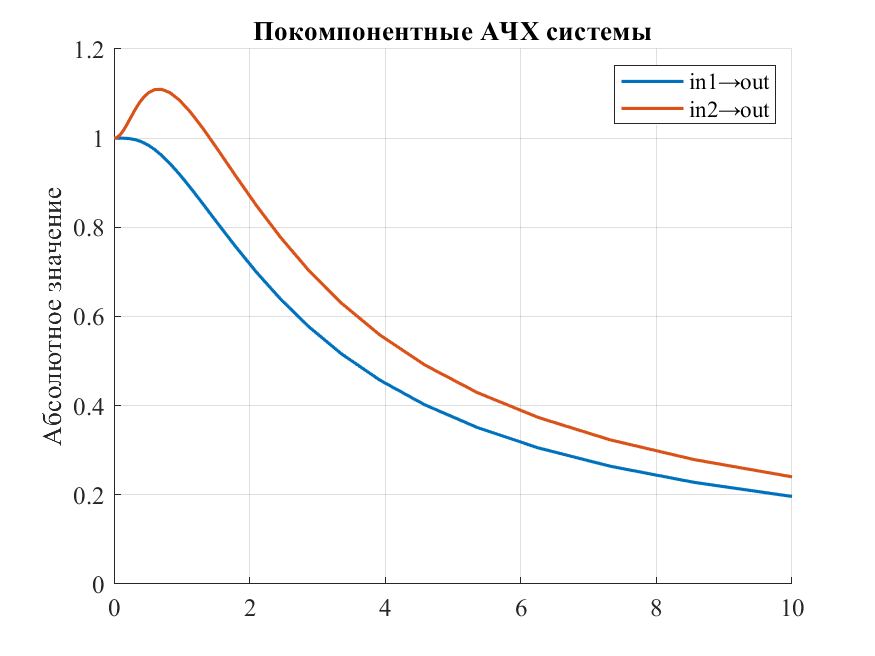
\includegraphics[width=0.8\textwidth]{freq_ampl_components3.png}
    \caption{Покомпонентные АЧХ}
  \end{figure}

\begin{figure}[ht]
  \centering
  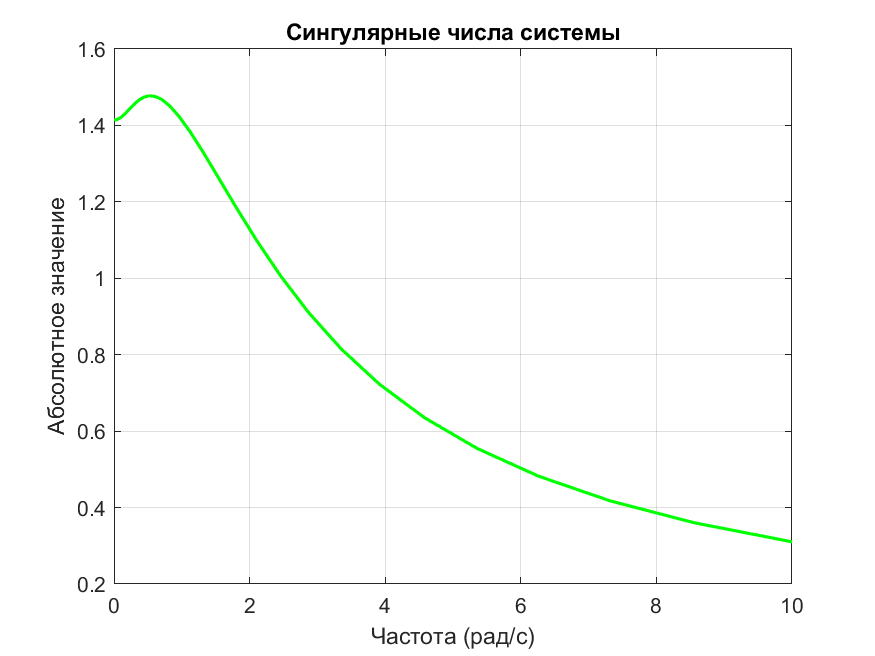
\includegraphics[width=0.8\textwidth]{singular_values3.png}
  \caption{Сингулярные числа}
\end{figure}
Нормы будем считать по следующим лекционным формулам, однако в \text{MATLAB} 
есть готовые реализации через функцию \text{norm}:
$$
    ||W||_{\mathcal{H}_2}  \approx 1.56
$$

$$
    ||W||_{\mathcal{H}_\infty}  \approx 1.47
$$

Выберем хорошую и плохую частоту $f_1, f_2$. 
Хорошей частотой для нас будет являться та, которая меньше увеличивает сигнал по амплитуде, и наоборот.
$$
    f_1 = 5.2 Hz, \tab f_2 = 0.6 Hz
$$

\subsection{Первое гармоническое возмушение}
\begin{figure}[ht]
    \centering
    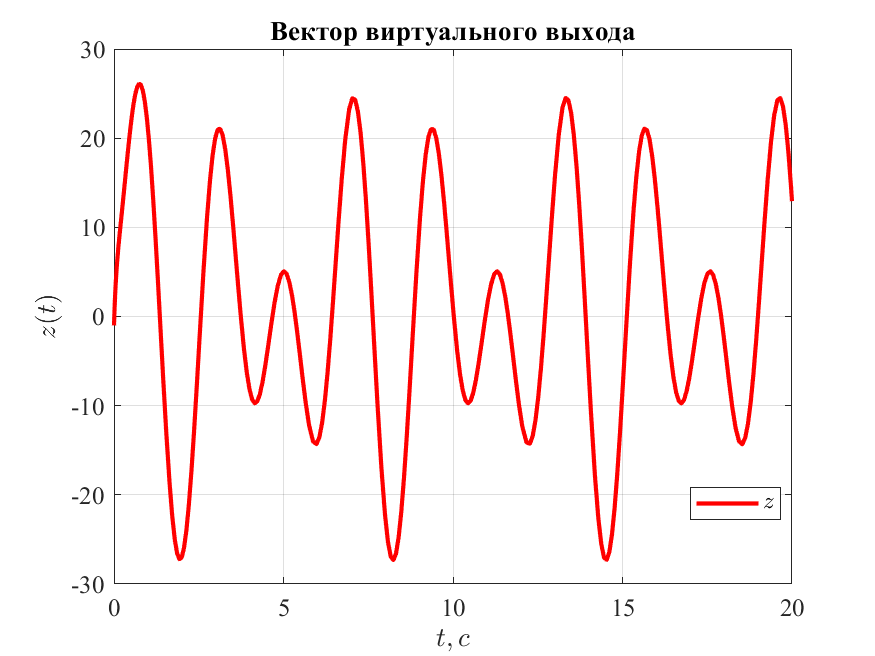
\includegraphics[width=0.8\textwidth]{z5.png}
    \caption{Моделирование -  регулируемый выход $z(t)$}
  \end{figure}

\newpage
\subsection{Второе гармоническое возмушение}
\begin{figure}[ht]
    \centering
    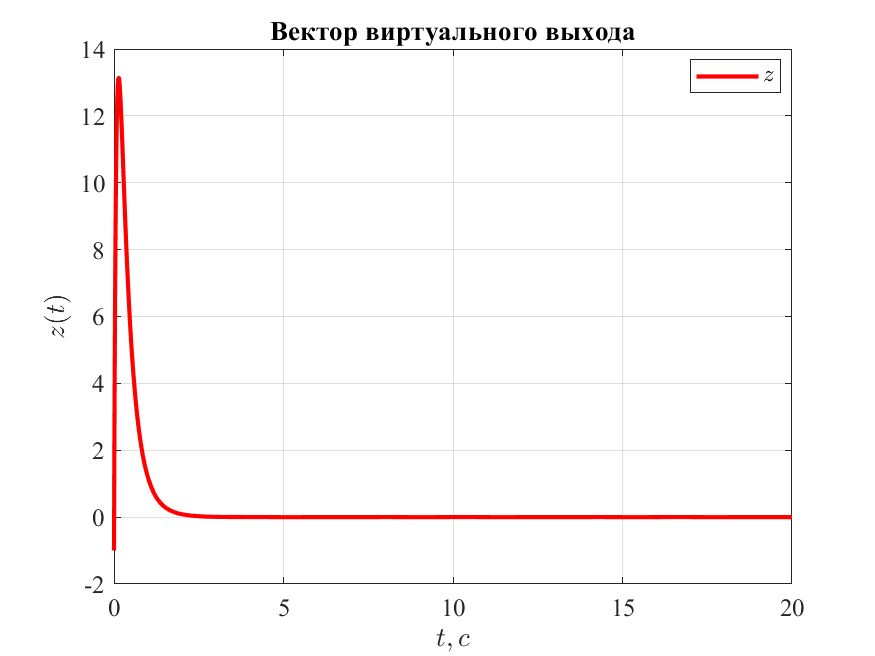
\includegraphics[width=0.8\textwidth]{z6.png}
    \caption{Моделирование -  регулируемый выход $z(t)$}
  \end{figure}

Как и в прошлых случаях, амплитуда регулируемого выхода $z(t)$ различаются по своему абсолютному значению в зависимости от выбранной частоты
внешних возмущений, наблюдатель в целом показывает те же результаты, что и в прошлом задании мы получили от наблюдения непосредственно за объектом. 
При синтезе такого наблюдателя мы гарантировали минимальность $||W||_{\mathcal{H}_2}$, 
также как и в прошлых экспериментах - пиковое сингулярное число системы действительно равняется $||W||_{\mathcal{H}_\infty}$.

\newpage
\subsection{Второй набор $(C_{Z2},D_{Z2})$}
Получим следующую матрицу регулятора и матрицу коррекции наблюдателя: 
$$
    K = \begin{bmatrix}
        -1.5 & -1.8 \\
    \end{bmatrix}, \tab 
    L = \begin{bmatrix} -1.46 \\ -0.34 \\ \end{bmatrix}
$$
Получим следующую передаточную матрицу системы:
$$
    W_{w\rightarrow z}(s) = \begin{bmatrix}\frac{1s^{3} + 4.8s^{2} + 6.91s + 4.5}{1s^{4} + 3.61s^{3} + 6.25s^{2} + 5.41s + 2.25} & \frac{-3.61s^{3} - 9.5s^{2} - 10.82s - 4.5}{1s^{4} + 3.61s^{3} + 6.25s^{2} + 5.41s + 2.25} \end{bmatrix}^T
$$


\begin{figure}[ht]
    \centering
    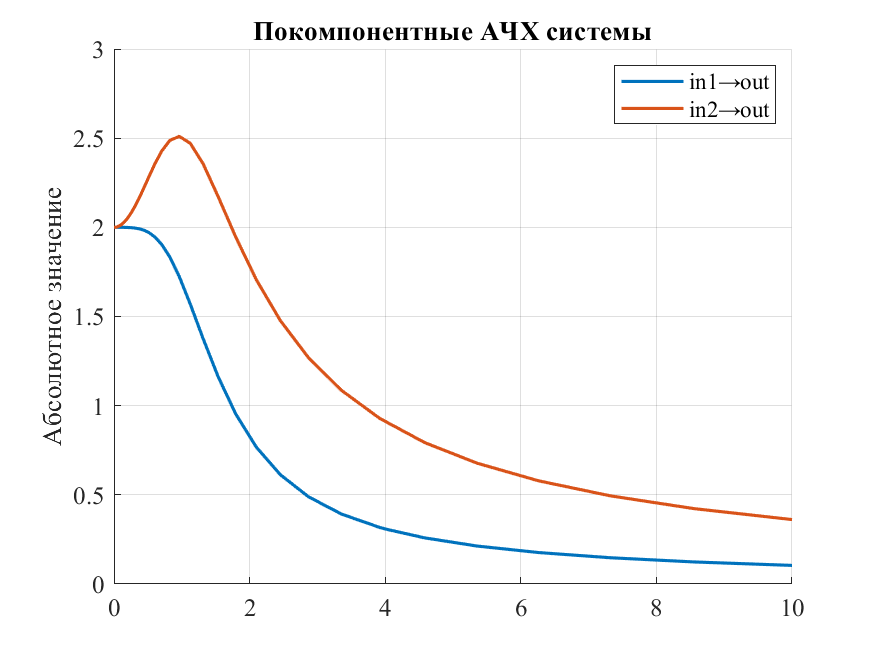
\includegraphics[width=0.8\textwidth]{freq_ampl_components4.png}
    \caption{Покомпонентные АЧХ}
  \end{figure}

\begin{figure}[ht]
  \centering
  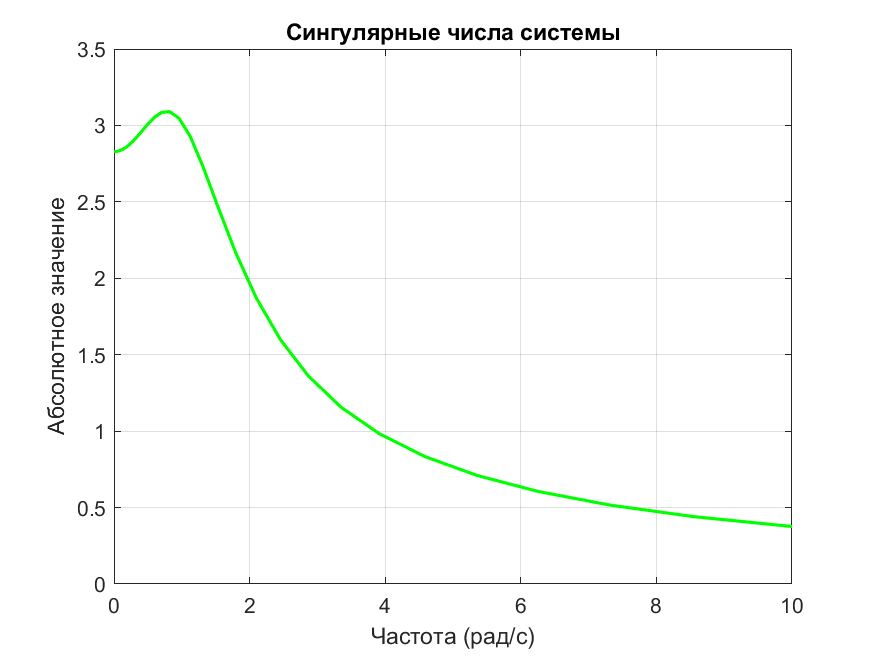
\includegraphics[width=0.8\textwidth]{singular_values4.png}
  \caption{Сингулярные числа}
\end{figure}
Нормы будем считать по следующим лекционным формулам, однако в \text{MATLAB} 
есть готовые реализации через функцию \text{norm}:
$$
    ||W||_{\mathcal{H}_2}   \approx 2.68
$$

$$
    ||W||_{\mathcal{H}_\infty}  \approx 3.09
$$

Выберем хорошую и плохую частоту $f_1, f_2$. 
Хорошей частотой для нас будет являться та, которая меньше увеличивает сигнал по амплитуде, и наоборот.
$$
    f_1 = 3.5 Hz, \tab f_2 = 0.85 Hz
$$

\subsection{Первое гармоническое возмушение}
\begin{figure}[ht]
    \centering
    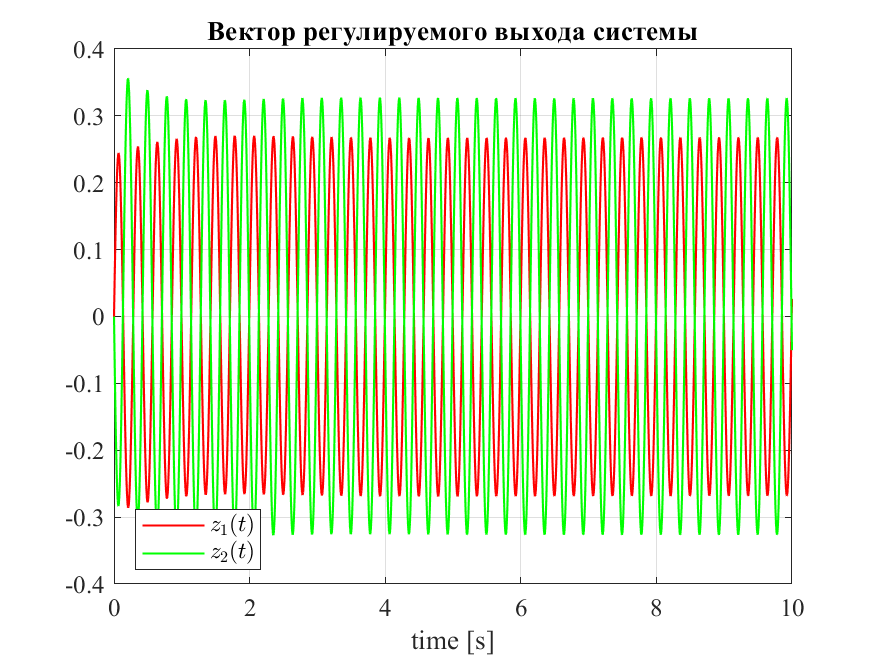
\includegraphics[width=0.8\textwidth]{z7.png}
    \caption{Моделирование -  регулируемый выход $z(t)$}
  \end{figure}

\subsection{Второе гармоническое возмушение}
\begin{figure}[ht]
    \centering
    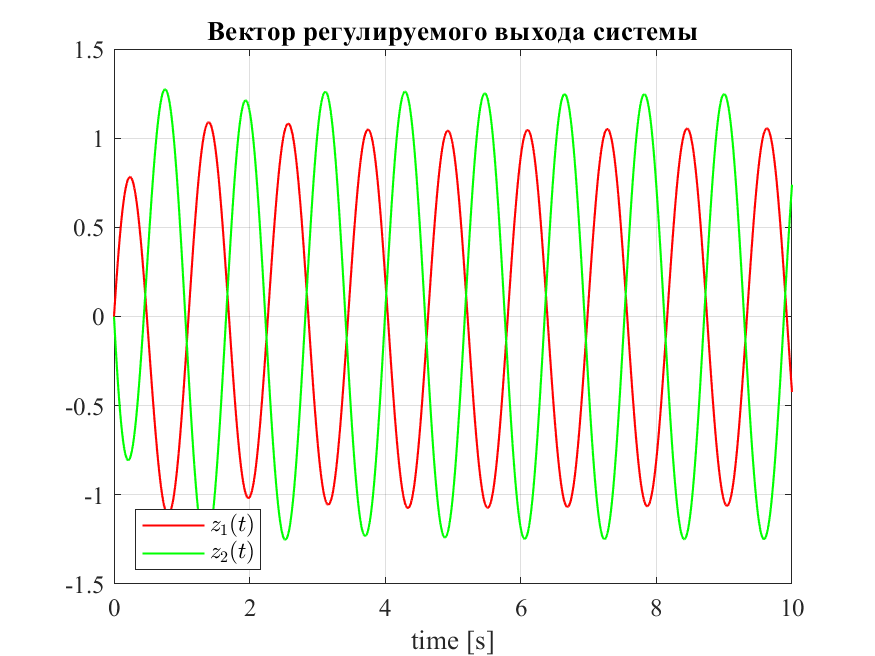
\includegraphics[width=0.8\textwidth]{z8.png}
    \caption{Моделирование -  регулируемый выход $z(t)$}
\end{figure}

Можно сделать выводы, аналогичные первому набору, только сейчас мы изменили немного "угол обзора" на ситуацию, поменяв матрицы $(C_Z,D_Z)$ регулируемого выхода.

\subsection{Вывод}
В этом задании мы синтезировали $\mathcal{H}_2$-регулятор по выходу, который нам позволил 
уменьшить АЧХ передаточной матрицы системы "в среднем", поэтому в результате мы не получили значительного 
приглушения $z(t)$ сигнала по амплитуде при выборе "плохой" частоты. 
Мы смогли удостовериться в этом при помощи моделирования.
\endinput